\section{Feed-Forward Neural Networks}
A feed-forward neural network is a function $h(\mathbf{x})$. To understand how it works, it's instructive to look at each part of its name in isolation.
\\\\
$h$ is called a \textbf{network} because it's a composition of $L$ \textbf{layers} of other functions $f_l$. Each $f_l$ receives input from $f_{l-1}$. For example if $L = 2$, then $h(\mathbf{x}) = f_2(f_1(\mathbf{x}))$. The number of layers $L$ is called the \textbf{depth} of the network. $f_L$ is called the \textbf{output layer}. The remaining functions $f_1$ to $f_{L-1}$ are called \textbf{hidden layers}. Each $f_l$ outputs a vector $\mathbf{z}_l$ of dimension $d_l$. The size of these vectors determine the \textbf{width} of the network. We denote the input to $f_1$ as $\mathbf{z}_0$, which is the input $\mathbf{x}$ to $h(\mathbf{x})$ with an added \textbf{bias} component, as described later in this section.
\\\\
The functions $f_1$ to $f_L$ are ordered by their index $l$. By ordered, we mean that the index of the innermost functions are smaller than the index of the outermost. $h$ is called a \textbf{feed-forward} network because each $f_l$ can receive input only from functions $f_i$ if $l > i$. In other words, its not possible for a function $f_l$ to feed its own output into itself, or any other function that it receives input from. Networks where this restriction is removed are called \textbf{recurrent neural networks}, and will be discussed in section \ref{rnns}.
\\\\
Finally $h$ is called a \textbf{neural} network since its design is loosely based on neurons in the brain \citep{goodfellow16}. Each component $z$ of the vector $\mathbf{z}_l$ can be seen as the output of a unit similar to a neuron. Each unit in layer $l$ receives input from units in layer $l-1$. The output $z_{l-1,v}$ of unit $v$ in layer $l-1$ is multiplied by a weight $w_{l,v,u}$ that gives the strength of the connection between unit $v$ in $l-1$ and unit $u$ in $l$. Unit $u$ sums all of the input it receives from units in layer $l-1$ to obtain its \textbf{activation} $a_{l,u} = \sum w_{l,v,u}z_{l-1,v}$. To compute its output $z_{l,u}$, it applies an \textbf{activation function} $\sigma(a_{l,u})$ to its activation.

Activation functions model the behaviour of biological neurons by outputting a signal only when the activation is above a certain threshold. To make it possible to learn this threshold for each unit using the same activation function, we introduce a special \textbf{bias} unit that always outputs 1. The index of the bias unit in layer $l$ is 0 by convention. Figure \ref{connection}. shows how a unit $u$ computes its output $z_{l,u}$ by combining the outputs of units in layer $l-1$.

\tikzstyle{neuron}=[circle,draw,minimum size=20pt,inner sep=0pt]
\tikzstyle{summation} = [square, minimum size=20pt,inner sep=0pt]
\tikzstyle{edge} = [draw,thick,-]
\tikzstyle{weight} = [font=\small]

\begin{figure}[h]
	\centering
	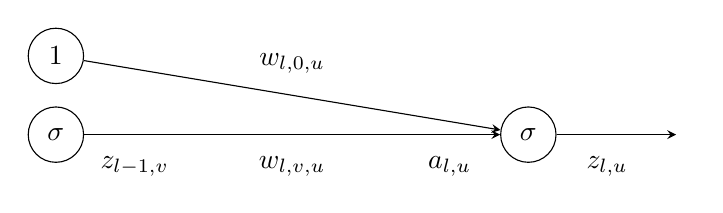
\begin{tikzpicture}[->, >=stealth, swap]
			\node [neuron] (sigma1) at (0,0) {$\sigma$};
			\node [neuron] (sigma2) at (6,0) {$\sigma$};
			\node [neuron] (bias1) at (0,1) {$1$};
			\node []       (z1)      at (1,-.4) {$z_{l-1,v}$};
			\node []       (w)     at (3,-.4) {$w_{l,v,u}$};
			\node []       (w)     at (3,.9) {$w_{l,0,u}$};
			\node []       (aw)   at (5,-.4) {$a_{l,u}$};
			\node []	   (empty) at (8,0) {};
			\node []       (z2)    at (7,-.4) {$z_{l,u}$};
		
			\draw (sigma1) edge (sigma2);
			\draw (sigma2) edge (empty);
			\draw (bias1) edge (sigma2);
	\end{tikzpicture}
	\caption{A visual representation of the connections between unit $v$ in layer $l-1$, the bias unit in $l-1$, and unit $u$ in layer $l$. The connection strength between these units is given by the weight $w_{l,v,u}$ between $v$ and $u$, and $w_{l,0,u}$ between the bias unit and $u$. The activation $a_{l,u}$ at unit $u$ is computed by $a_{l,u} = w_{l,v,u}z_{l-i,v} + w_{l,0,u}$. The output $z_{l,u}$ of unit $u$ is given by $z_{l,u} = \sigma(a_{l,u})$}
	\label{connection}
\end{figure}
\noindent
Keeping track of the indices $l$, $u$ and $v$ quickly becomes confusing. By collecting all of the weights of connections going into unit $u$ in layer $l$ in a vector $\mathbf{w}_{l,u}$, the activation at unit $u$ can be computed as a dot product $a_{l,u} = {\mathbf{w}_{l,u}}^T\mathbf{z}_{l-1}$. Moreover, we can compute the entire vector $\mathbf{a}_l$ of activations at layer $l$, by organising the weight vectors $\mathbf{w}_{l,u}$ in a matrix $\mathbf{W}_l = [\mathbf{w}_{l,1}\, \dots\, \mathbf{w}_{l,d_l}]^T$, which leads to $\mathbf{a}_l = \mathbf{W}_l\mathbf{z}_{l-1}$.
\\\\
By gathering the weights in matrices $\mathbf{W}_l$, we have simplified our view of $h$ into a composition of matrix-vector products and element-wise application of activation functions. Figure \ref{neural_network} shows the parallel views of neural networks as networks of units and matrix-vector operations.

\begin{figure}[h]
	\centering
	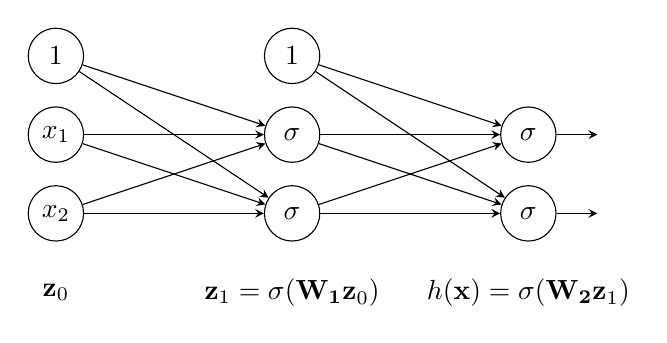
\begin{tikzpicture}[->, >=stealth, swap]
		\node [neuron] (bias0)   at (0, 2)  {1};
		\node [neuron] (x1)      at (0, 1)  {$x_1$};
		\node [neuron] (x2)      at (0, 0)  {$x_2$};
		\node []       (x)       at (0,-1)  {$\mathbf{z}_0$};
		\node [neuron] (bias1)   at (3, 2)  {1}; 
		\node [neuron] (sigma11) at (3, 1)  {$\sigma$};
		\node [neuron] (sigma12) at (3, 0)  {$\sigma$};
		\node []       (layer1)  at (3,-1)  {$\mathbf{z}_1 = \sigma(\mathbf{W_1 z}_0)$};
		\node [neuron] (sigma21) at (6, 1)  {$\sigma$};
		\node [neuron] (sigma22) at (6, 0)  {$\sigma$};
		\node []       (layer2)  at (6,-1)  {$h(\mathbf{x}) = \sigma(\mathbf{W_2 z}_1)$};
		\node []	   (empty1)  at (7, 1) {};
		\node []       (empty2)  at (7, 0) {};   
		
		
		\draw (bias0)   edge (sigma11);
		\draw (x1)      edge (sigma11);
		\draw (x2)      edge (sigma11);
		\draw (bias0)   edge (sigma12);
		\draw (x1)      edge (sigma12);
		\draw (x2)      edge (sigma12);
		\draw (bias1)   edge (sigma21);
		\draw (sigma11) edge (sigma21);
		\draw (sigma12) edge (sigma21);
		\draw (bias1)   edge (sigma22);
		\draw (sigma11) edge (sigma22);
		\draw (sigma12) edge (sigma22);
		\draw (sigma21) edge (empty1);
		\draw (sigma22) edge (empty2);
	\end{tikzpicture}
	\caption{A visual representation of $h(\mathbf{x}) = f_2(f_1(\mathbf{x}))$. The activation at each layer $\mathbf{a}_l$ is computed by $\mathbf{W}_l\mathbf{z}_{l-1}$. The output at each layer is computed by element-wise application of the activation function of $\sigma(\mathbf{a}_l)$.}
	\label{neural_network}
\end{figure}
\noindent
We now have all the components we need to specify $\mathcal{H}$ as a set of neural networks. The set is defined by the depth of the networks $L$, the number of units in each layer $d_l$ , and the activation function $\sigma$.
For a particular $L$, $d_l$, and $\sigma$, each $h \in \mathcal{H}$ is given by the set of all its weights $\mathcal{W} = \{\mathbf{W}_1\, \dots \, \mathbf{W}_L\}$. We sometimes make the dependence of $h$ on $\mathcal{W}$  explicit by using the notation $h(\mathbf{x}; \mathcal{W})$ which means \textit{the function $h$ parameterised by $\mathcal{W}$}. In the next section we discuss how to choose the activation functions at the layers of the network.
\subsection{Activation Functions}
\subsection{Objective Function}